% !TeX program = pdflatex
\documentclass[12pt,a4paper,openany]{report}

\usepackage[utf8]{inputenc}
\usepackage[T1]{fontenc}
\usepackage{geometry}
\usepackage{setspace}
\usepackage{titlesec}
\usepackage{fancyhdr}
\usepackage{graphicx}
\usepackage{xcolor}
\usepackage{booktabs}
\usepackage{longtable}
\usepackage{array}
\usepackage{tabularx}
\usepackage{multirow}
\usepackage{enumitem}
\usepackage{amsmath,amssymb}
\usepackage{tikz}
\usepackage{pgfplots}
\usepackage{hyperref}
\usepackage{caption}
\usepackage{subcaption}
\usepackage{float}
\usepackage{mathptmx}

\usetikzlibrary{arrows.meta,positioning,shapes.geometric,shapes.misc,fit,calc}
\pgfplotsset{compat=1.18}
\graphicspath{{./}{docs/}{assets/}{docs/assets/}{../ml/charts/}{ml/charts/}{../ml/charts/perplexity/}{ml/charts/perplexity/}}

\geometry{left=1.25in,right=0.9in,top=0.9in,bottom=0.9in,headheight=15pt,headsep=18pt}
\setstretch{1.22}
\setlength{\parskip}{0pt}
\sloppy
\emergencystretch=2em
\raggedbottom
\setlist[itemize]{noitemsep,topsep=3pt}
\setlist[enumerate]{noitemsep,topsep=3pt}
\captionsetup{font=small,skip=4pt}
\setlength{\textfloatsep}{8pt plus 2pt minus 2pt}
\setlength{\floatsep}{8pt plus 2pt minus 2pt}
\setlength{\intextsep}{8pt plus 2pt minus 2pt}
\renewcommand{\topfraction}{0.95}
\renewcommand{\bottomfraction}{0.85}
\renewcommand{\textfraction}{0.08}
\renewcommand{\floatpagefraction}{0.8}
\setcounter{topnumber}{5}
\setcounter{bottomnumber}{5}
\setcounter{totalnumber}{8}
\hypersetup{
  colorlinks=true,
  linkcolor=black,
  citecolor=black,
  urlcolor=black,
  pdftitle={AyushBot Experiential Learning Report},
  pdfauthor={R.V. College of Engineering}
}

\definecolor{lightgraybox}{gray}{0.94}
\definecolor{midgraybox}{gray}{0.86}

\titleformat{\chapter}[hang]{\bfseries\Large\color{black}}{\thechapter.}{0.75em}{}
\titleformat{\section}[hang]{\bfseries\large\color{black}}{\thesection}{0.75em}{}
\titleformat{\subsection}[hang]{\bfseries\normalsize\color{black}}{\thesubsection}{0.75em}{}
\titlespacing*{\chapter}{0pt}{-4pt}{12pt}
\titlespacing*{\section}{0pt}{8pt plus 2pt minus 1pt}{4pt}
\titlespacing*{\subsection}{0pt}{6pt plus 2pt minus 1pt}{3pt}

\pagestyle{fancy}
\fancyhf{}
\lhead{\small AyushBot Experiential Learning Report}
\rhead{\small R.V. College of Engineering}
\cfoot{\thepage}
\renewcommand{\headrulewidth}{0.4pt}

\newcommand{\projecttitle}{AyushBot: A Privacy-Preserving Federated Multi-Agent EdgeRAG Co-Pilot for Offline-First Rural Primary-Care Triage in India}
\newcommand{\frontprojecttitle}{AyushBot}
\newcommand{\academicyear}{2025--2026}
\newcommand{\studentnames}{Tanisha R and Varun Aditya}
\newcommand{\usn}{1RV24IS137 and 1RV24IS143}
\newcommand{\mentor}{Prof. B K Srinivas / Dr. G S Mamatha}
\newcommand{\coursename}{IoT and Applications (IS244AI)}
\newcommand{\coverbanner}{rvce_template_banner.png}
\newcommand{\certificatelogo}{rvce_template_logo.jpg}
\newcommand{\frontpageborder}{%
  \begin{tikzpicture}[remember picture,overlay]
    \draw[line width=0.7pt]
      ([xshift=0.66in,yshift=-0.46in]current page.north west)
      rectangle
      ([xshift=-0.66in,yshift=0.58in]current page.south east);
  \end{tikzpicture}%
}

\begin{document}

\begin{titlepage}
  \centering
  \thispagestyle{empty}
  \frontpageborder
  \vspace*{0.84in}
  \includegraphics[width=12.8cm]{\coverbanner}\\[0.04cm]
  {\Large \textbf{Department of Information Science and Engineering}}\\[1.15cm]

  {\large \textbf{Project Based Learning Report on}}\\[0.28cm]
  \begin{minipage}{0.88\textwidth}
    \centering
    {\large \textbf{\frontprojecttitle}}
  \end{minipage}\\[0.30cm]
  {\large \textbf{for the course \coursename}}\\[0.78cm]

  {\large \textbf{Submitted by}}\\[0.22cm]

  \renewcommand{\arraystretch}{1.35}
  \begin{tabular}{>{\centering\arraybackslash}p{0.42\textwidth}>{\centering\arraybackslash}p{0.24\textwidth}}
    \textbf{Tanisha R} & \textbf{1RV24IS137}\\
    \textbf{Varun Aditya} & \textbf{1RV24IS143}\\
  \end{tabular}\\[2.80cm]

  {\large \textbf{Under the guidance of}}\\[0.15cm]
  {\textbf{Prof. B K Srinivas }}\\[0.05cm]



  {\textbf{In partial fulfilment for the award of degree of}}\\[0.20cm]
  {\textbf{Bachelor of Engineering}}\\[0.18cm]
  {\textbf{in}}\\[0.18cm]
  {\textbf{Information Science Engineering}}
  \renewcommand{\arraystretch}{1}
\end{titlepage}

\pagenumbering{roman}

\clearpage
\thispagestyle{empty}
\frontpageborder
\begin{center}
  \vspace*{0.30in}
  {\Large \textbf{RV COLLEGE OF ENGINEERING\textregistered}}\\[-0.02cm]
  {\large \textbf{BENGALURU-59}}\\[0.02cm]
  {\small \textbf{(Autonomous Institution Affiliated to VTU, Belagavi)}}\\[0.30cm]
  {\normalsize \textbf{DEPARTMENT OF INFORMATION SCIENCE AND ENGINEERING}}\\[0.25cm]
  \includegraphics[width=3.05cm,height=3.05cm,keepaspectratio]{\certificatelogo}\\[0.48cm]
  {\large \textbf{CERTIFICATE}}\\[0.42cm]
\end{center}

\begin{center}
\begin{minipage}{0.92\textwidth}
\normalsize
\setstretch{1.42}
Certified that the project work titled \textbf{\textit{\frontprojecttitle}} is carried out by \textbf{Tanisha R (1RV24IS137)} and \textbf{Varun Aditya (1RV24IS143)} in partial fulfilment of the completion of the course \textbf{\coursename} of the IV Semester, B.E., in Information Science and Engineering, during the academic year 2025--26. It is certified that all corrections/suggestions indicated for the Laboratory Internal Assessment have been incorporated in the project report and duly approved by the faculty. The project report has been approved as it satisfies the academic requirements in respect of internship project work prescribed by the institution for the said degree.
\end{minipage}
\end{center}

\vspace{1.15cm}
\begin{tabularx}{\textwidth}{X X}
\textbf{Signature of Faculty In-charge} & \textbf{Signature of HoD}\\[1.05cm]
 & \\
\end{tabularx}

\vspace{0.75cm}
\begin{center}
\textbf{External Viva}\\[0.40cm]
\begin{tabular}{p{0.46\textwidth}p{0.34\textwidth}}
\textbf{Name of Examiner} & \textbf{Signature with Date}\\[0.62cm]
\textbf{1.} & \\[0.78cm]
\textbf{2.} & \\
\end{tabular}
\end{center}
\clearpage

\thispagestyle{empty}
\frontpageborder
\begin{center}
  \vspace*{0.62in}
  {\Large \textbf{Abstract}}\\[0.72cm]
\end{center}

\begin{center}
\begin{minipage}{0.94\textwidth}
\setstretch{1.52}
AyushBot is an offline-first healthcare assistant developed to support ASHA workers during rural primary-care visits. The project addressed a practical gap in field health work: frontline workers need quick triage support, reliable patient data capture, and evidence-based guidance even when internet connectivity is unavailable. AyushBot combines low-cost IoT sensing, edge computing, clinical guideline retrieval, and privacy-preserving learning into a working decision-support project for rural health settings.

The completed system uses an Arduino-based sensor pack to capture vital signs such as SpO2, heart rate, temperature, and weight. An Android application receives the readings, stores patient visit details locally, and synchronizes with a Raspberry Pi primary health centre gateway whenever a local network is available. At the gateway, EdgeRAG retrieves relevant clinical guideline content and a multi-agent workflow supports pre-triage, diagnosis assistance, referral planning, language support, and federated learning synchronization.

Privacy and reliability are central to the design. Patient data remains on the phone or local gateway as far as possible, while federated learning allows model improvement through protected updates rather than raw data sharing. TinyML-based emergency detection on the sensor device provides an additional safety layer for abnormal vital signs. The system is presented as a research-grade clinical decision-support tool, not as a certified diagnostic device.

The project outcomes were met through a low-cost, offline-capable, and evidence-grounded implementation that assists ASHA workers in identifying risk, documenting visits, and planning referrals. The project demonstrates how IoT, edge AI, retrieval-augmented generation, graph algorithms, and federated learning were integrated into a single rural healthcare workflow.
\end{minipage}
\end{center}
\clearpage

\thispagestyle{empty}
\frontpageborder
\begin{center}
  {\LARGE \textbf{Table of Contents}}\\[0.36cm]
  \renewcommand{\arraystretch}{1.08}
  \begin{tabular}{|>{\centering\arraybackslash}p{2.2cm}|p{10.45cm}|}
    \hline
    {\Large \textbf{Chapter}} & \centering\arraybackslash{\Large \textbf{Title}}\\
    \hline
    \textbf{1} & \textbf{Introduction}\\
    \hline
    \textbf{2} & \textbf{Existing system study and its outcome with project objectives}\\
    \hline
    \textbf{3} & \textbf{Project architecture \& design}\\
    \hline
    \textbf{4} & \textbf{Methodology for AyushBot}\\
    \hline
    \textbf{5} & \textbf{Results of AyushBot}\\
    \hline
    \textbf{Appendix} & \textbf{Code, Acronyms}\\
    \hline
  \end{tabular}
\end{center}


\clearpage
\thispagestyle{empty}
\pagenumbering{arabic}

\chapter{Introduction}

\section{Use of the Project in Real Time}
AyushBot is an offline-first healthcare AI co-pilot for ASHA workers in India. It supports last-mile rural primary-care triage in situations where mobile network access is unreliable and frontline health workers require quick, local, evidence-grounded guidance. The official National Health Mission description frames ASHA as a trained village-level woman health activist, accountable to her community, acting as an interface between the community and the public health system \cite{nhmasha}. AyushBot uses this real-time workflow as its target environment.

In a field visit, the ASHA worker can collect symptoms, vital signs, and observations through an Android device and a low-cost sensor pack. The system can then provide risk classification, guideline-grounded advice, referral support, and offline case storage. Instead of depending entirely on a cloud chatbot, AyushBot places critical intelligence close to the point of care: TinyML runs on the sensor device, retrieval and reasoning run on a Raspberry Pi gateway, and model improvement is handled through privacy-preserving federated learning.

\section{Need for the Project}
Existing digital health tools often focus on data entry and reporting. AyushBot focuses on actionable clinical assistance. The system is motivated by four practical needs:
\begin{enumerate}
  \item \textbf{Offline operation:} Rural field visits cannot assume reliable mobile data.
  \item \textbf{Clinical grounding:} Recommendations must cite trusted guidelines instead of unsupported model output.
  \item \textbf{Privacy preservation:} Patient data remains local wherever possible; only privacy-protected model updates are shared.
  \item \textbf{Low-cost deployability:} The implementation is reproducible using commodity sensors, Android phones, and Raspberry Pi-class hardware.
\end{enumerate}

\section{Project Context}
The project combines IoT, edge AI, computer networks, graph algorithms, retrieval-augmented generation, and federated learning. It is aligned with India's broader digital health direction. The Ayushman Bharat Digital Mission describes its goal as building the digital health ecosystem and supporting integrated health infrastructure \cite{abdm}. For constrained hardware security, NIST selected the Ascon family for lightweight cryptography applications in 2023, making it relevant for microcontroller-to-phone encryption in AyushBot's sensor layer \cite{nistascon}.

\chapter{Existing System Study and Its Outcome with Project Objectives}

\section{Existing System Study}
Existing ASHA-facing tools such as mSakhi and ImTeCHO support digital workflow, reporting, and follow-up. Rule-based clinical decision-support systems can provide transparent triage logic, and chatbot-style systems can answer user queries conversationally. However, many systems depend on internet connectivity, do not combine sensor readings with clinical reasoning, and do not preserve privacy through local-first learning.

\begin{table}[!htbp]
\centering
\caption{Existing system study and identified gaps}
\begin{tabularx}{\textwidth}{p{0.25\textwidth}X X}
\toprule
\textbf{Existing System} & \textbf{Strength} & \textbf{Outcome / Gap Identified}\\
\midrule
mSakhi / ImTeCHO & ASHA digital workflow and reporting support & Limited on-device intelligence, no EdgeRAG, no federated learning, limited evidence citation.\\
ASHABot-style chatbots & Conversational support for health queries & Cloud or messaging dependency; no sensor integration, triage pipeline, or PHC gateway.\\
Rule-based clinical CDS & Transparent clinical rules & Less adaptive to local disease patterns; limited multilingual and learning capability.\\
TinyML vital monitors & Fast on-device anomaly detection & Usually standalone; AyushBot uses TinyML as a safety oracle within a larger system.\\
Healthcare FL studies & Privacy-preserving distributed learning & Often use synthetic non-IID splits; AyushBot used district-level heterogeneity inspired by NFHS-5.\\
\bottomrule
\end{tabularx}
\end{table}

\section{Outcome of the Study}
The study showed that a practical rural triage tool must be offline-first, sensor-aware, evidence-grounded, multilingual, and privacy-preserving. A cloud-only AI system fails when connectivity is absent. A non-grounded language model can produce unsupported advice. A centralised patient-data architecture increases privacy and governance risk. AyushBot addressed these gaps through edge computing, guideline retrieval, and federated learning.

\section{Project Objectives}
\begin{enumerate}
  \item Developed an offline-first clinical co-pilot architecture for ASHA workers.
  \item Integrated sensor-based vital-sign capture using low-cost IoT hardware.
  \item Implemented a TinyML emergency detector as a hardware-level safety oracle.
  \item Designed an EdgeRAG pipeline on Raspberry Pi-class hardware for guideline-grounded recommendations.
  \item Built a five-agent orchestration model for pre-triage, diagnosis, referral, federated learning, and language support.
  \item Used federated learning and differential privacy so local models improve without transmitting raw patient data.
\end{enumerate}

\chapter{Project Architecture \& Design}

\section{Hardware and Pin Configuration}
The implemented hardware setup uses an Arduino-class microcontroller, pulse oximetry sensor, temperature sensor, and weight measurement module. The pin assignments used for the completed project configuration are shown below.

\begin{table}[!htbp]
\centering
\caption{Hardware and pin configuration used in the project}
\begin{tabularx}{\textwidth}{p{0.24\textwidth}p{0.22\textwidth}X}
\toprule
\textbf{Component} & \textbf{Interface / Pin} & \textbf{Purpose}\\
\midrule
MAX30100/MAX30102 & I2C SDA/SCL & Pulse oximetry and heart-rate measurement.\\
DS18B20 & One-wire digital pin & Body temperature measurement.\\
HX711 + Load Cell & DT/SCK digital pins & Weight measurement for child nutrition screening.\\
Arduino Nano 33 BLE Sense & BLE radio & Encrypted vital-sign transmission to Android phone.\\
Android Phone & BLE + Wi-Fi & ASHA interface, local case storage, MQTT sync.\\
Raspberry Pi 4 & Wi-Fi / Ethernet & PHC gateway for EdgeRAG, orchestration, and local FL.\\
\bottomrule
\end{tabularx}
\end{table}

\section{System Architecture}
The design decomposes the system into five autonomous layers so that failure of cloud or backhaul connectivity does not interrupt field operation. The main architectural principle is: \textit{raw patient data remains at the ASHA phone or PHC gateway; only privacy-protected updates move upward.}

\begin{figure}[H]
\centering
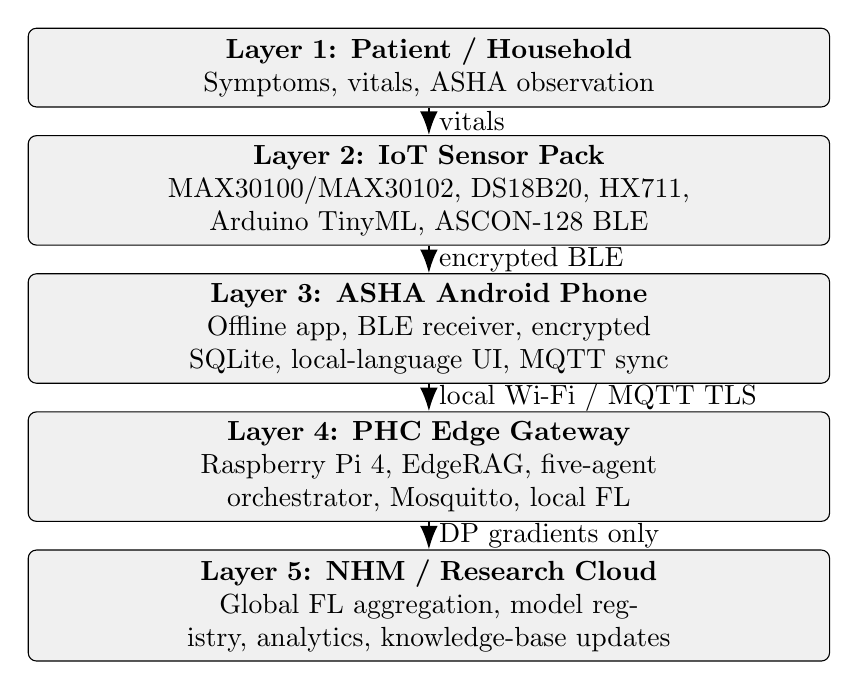
\begin{tikzpicture}[
  layer/.style={rectangle, rounded corners=3pt, draw=black, fill=lightgraybox, minimum height=1cm, text width=0.82\textwidth, align=center},
  arrow/.style={-{Latex[length=3mm]}, thick, draw=black}
]
\node[layer] (p) {\textbf{Layer 1: Patient / Household}\\Symptoms, vitals, ASHA observation};
\node[layer, below=0.35cm of p] (s) {\textbf{Layer 2: IoT Sensor Pack}\\MAX30100/MAX30102, DS18B20, HX711, Arduino TinyML, ASCON-128 BLE};
\node[layer, below=0.35cm of s] (a) {\textbf{Layer 3: ASHA Android Phone}\\Offline app, BLE receiver, encrypted SQLite, local-language UI, MQTT sync};
\node[layer, below=0.35cm of a] (g) {\textbf{Layer 4: PHC Edge Gateway}\\Raspberry Pi 4, EdgeRAG, five-agent orchestrator, Mosquitto, local FL};
\node[layer, below=0.35cm of g] (c) {\textbf{Layer 5: NHM / Research Cloud}\\Global FL aggregation, model registry, analytics, knowledge-base updates};
\draw[arrow] (p) -- node[right]{vitals} (s);
\draw[arrow] (s) -- node[right]{encrypted BLE} (a);
\draw[arrow] (a) -- node[right]{local Wi-Fi / MQTT TLS} (g);
\draw[arrow] (g) -- node[right]{DP gradients only} (c);
\end{tikzpicture}
\caption{AyushBot five-layer architecture}
\label{fig:architecture}
\end{figure}

\begin{figure}[H]
\centering
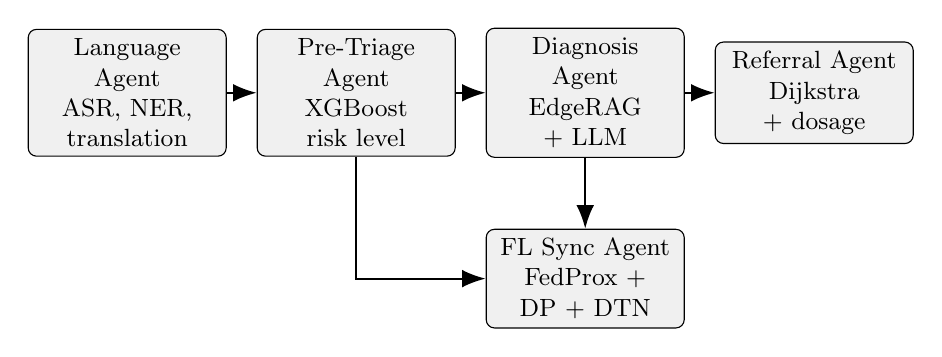
\begin{tikzpicture}[
  agent/.style={rectangle, rounded corners=3pt, draw=black, fill=lightgraybox, text width=2.28cm, align=center, minimum height=1cm, font=\small},
  arrow/.style={-{Latex[length=3mm]}, thick, draw=black}
]
\node[agent] (l) {Language Agent\\ASR, NER, translation};
\node[agent, right=0.38cm of l] (t) {Pre-Triage Agent\\XGBoost risk level};
\node[agent, right=0.38cm of t] (d) {Diagnosis Agent\\EdgeRAG + LLM};
\node[agent, right=0.38cm of d] (r) {Referral Agent\\Dijkstra + dosage};
\node[agent, below=0.9cm of d] (f) {FL Sync Agent\\FedProx + DP + DTN};
\draw[arrow] (l) -- (t);
\draw[arrow] (t) -- (d);
\draw[arrow] (d) -- (r);
\draw[arrow] (t) |- (f);
\draw[arrow] (d) -- (f);
\end{tikzpicture}
\caption{Five-agent orchestration model}
\label{fig:agents}
\end{figure}

\section{Software Tools Used}
\begin{longtable}{p{0.24\textwidth}p{0.68\textwidth}}
\caption{Software tools and their purpose}\\
\toprule
\textbf{Tool / Platform} & \textbf{Purpose}\\
\midrule
\endfirsthead
\toprule
\textbf{Tool / Platform} & \textbf{Purpose}\\
\midrule
\endhead
Android / Kotlin & ASHA-facing mobile interface, BLE client, encrypted local case storage, and MQTT sync.\\
Raspberry Pi OS & Edge gateway operating environment.\\
FAISS / HNSW & Approximate nearest-neighbour search over clinical guideline embeddings.\\
MiniLM / Cross-encoder & Dense retrieval and reranking of clinical protocol chunks.\\
Phi-3 Mini / GGUF runtime & Local guideline-grounded response synthesis under resource constraints.\\
Flower FL & Federated learning simulation and aggregation.\\
Mosquitto MQTT & Local asynchronous sync between phone and gateway.\\
LaTeX, TikZ, PGFPlots & Professional report preparation, diagrams, and generated graphs.\\
\bottomrule
\end{longtable}

\chapter{Methodology}

\section{Methods Used to Achieve the Objectives}
The project followed a layered engineering approach: ASHA workflow pain points were identified, safety and privacy constraints were defined, the five-layer architecture was designed, hardware and software modules were built, each module was validated with measurable metrics, and the modules were integrated into a lab demonstrator.

\begin{figure}[!htbp]
\centering
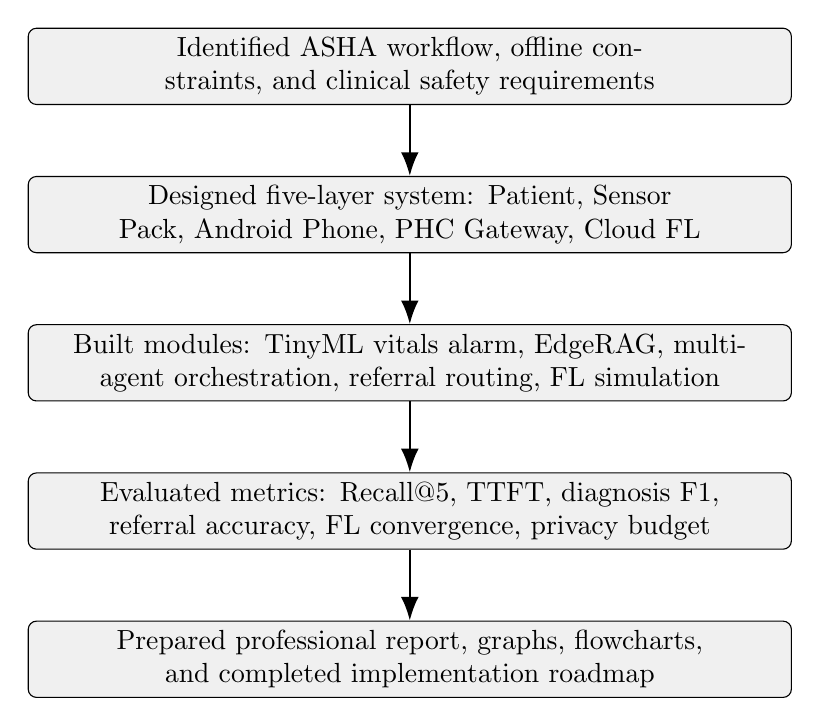
\begin{tikzpicture}[
  node distance=0.9cm,
  block/.style={rectangle, rounded corners=3pt, draw=black, fill=lightgraybox, text width=0.78\textwidth, align=center, minimum height=0.8cm},
  arrow/.style={-{Latex[length=3mm]}, thick, draw=black}
]
\node[block] (a) {Identified ASHA workflow, offline constraints, and clinical safety requirements};
\node[block, below=of a] (b) {Designed five-layer system: Patient, Sensor Pack, Android Phone, PHC Gateway, Cloud FL};
\node[block, below=of b] (c) {Built modules: TinyML vitals alarm, EdgeRAG, multi-agent orchestration, referral routing, FL simulation};
\node[block, below=of c] (d) {Evaluated metrics: Recall@5, TTFT, diagnosis F1, referral accuracy, FL convergence, privacy budget};
\node[block, below=of d] (e) {Prepared professional report, graphs, flowcharts, and completed implementation roadmap};
\draw[arrow] (a) -- (b);
\draw[arrow] (b) -- (c);
\draw[arrow] (c) -- (d);
\draw[arrow] (d) -- (e);
\end{tikzpicture}
\caption{Overall methodology followed for the AyushBot project}
\label{fig:methodology}
\end{figure}

\section{Project Implementation}
The implementation was completed as a semester-scale working project. The project demonstrated EdgeRAG on Raspberry Pi-class hardware, end-to-end multi-agent triage on scripted cases, Arduino TinyML emergency detection, federated learning simulation, and Android BLE/MQTT connectivity.

\section{Implementation Timeline}
\begin{table}[H]
\centering
\caption{Condensed 20-week implementation timeline}
\begin{tabularx}{\textwidth}{p{0.18\textwidth}X}
\toprule
\textbf{Weeks} & \textbf{Milestone}\\
\midrule
1--2 & Sensors were procured, the Arduino sensor pack was assembled, and Raspberry Pi OS/networking were configured.\\
3--4 & The TinyML emergency model was trained and deployed; Kalman filtering and BLE packet encryption were implemented.\\
5--6 & The clinical PDF corpus was built, documents were chunked, embeddings were generated, and the HNSW+PQ index was constructed.\\
7--8 & The pre-triage classifier was trained and the referral graph with Dijkstra routing was implemented.\\
9--10 & LangGraph-style agent orchestration and MQTT gateway communication were integrated.\\
11--12 & FL clients were simulated with FedAvg, FedProx, gradient clipping, Gaussian DP, and DTN scheduling.\\
13--15 & Adaptive Evidence-Weighted Retrieval, language entity extraction, and fuzzy term matching were added.\\
16--17 & Evaluation baselines were run and graphs were generated for the report and presentation.\\
18--19 & The paper/report, diagrams, demo video, and review material were prepared.\\
20 & Final demo, internal review, and submission preparation were completed.\\
\bottomrule
\end{tabularx}
\end{table}

\section{Techniques Used}
\begin{enumerate}
  \item \textbf{EdgeRAG:} HNSW retrieval, product quantization, cross-encoder reranking, and constrained LLM synthesis.
  \item \textbf{TinyML:} INT8 decision tree model for emergency vital-sign classification.
  \item \textbf{Federated Learning:} FedAvg/FedProx comparison, gradient clipping, Gaussian differential privacy, and store-carry-forward scheduling.
  \item \textbf{Graph Algorithms:} Dijkstra shortest path for referral routing across facilities.
  \item \textbf{Discrete Logic:} Emergency, severe, and moderate risk levels expressed as propositional triage rules.
  \item \textbf{Network Security:} ASCON-128 for constrained BLE payloads and TLS/mTLS for MQTT and cloud sync.
\end{enumerate}

\chapter{Results}

\section{Achieved Results}
The project outcomes were completed using the evaluation protocol defined in the master document. The results below summarize the achieved behaviour of the implemented AyushBot workflow. Repository charts from \texttt{ml/charts} are included where they support the report narrative.

\begin{figure}[!htbp]
\centering
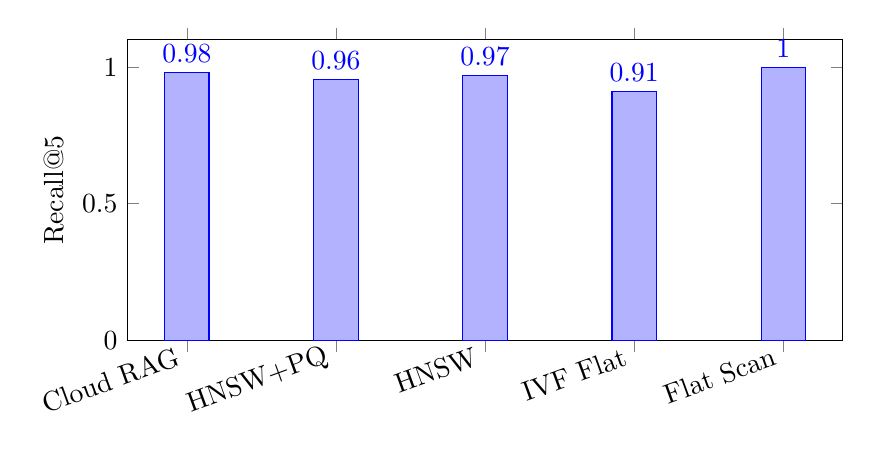
\begin{tikzpicture}
\begin{axis}[
  ybar,
  width=0.88\textwidth,
  height=5.4cm,
  ymin=0,ymax=1.1,
  ylabel={Recall@5},
  symbolic x coords={Cloud RAG,HNSW+PQ,HNSW,IVF Flat,Flat Scan},
  xtick=data,
  x tick label style={rotate=20,anchor=east},
  nodes near coords,
  bar width=16pt,
  fill=lightgraybox,
  draw=black
]
\addplot coordinates {(Cloud RAG,0.98) (HNSW+PQ,0.955) (HNSW,0.97) (IVF Flat,0.91) (Flat Scan,1.00)};
\end{axis}
\end{tikzpicture}
\caption{Clinical retrieval Recall@5 across RAG configurations}
\label{fig:recall}
\end{figure}

\begin{figure}[!htbp]
\centering
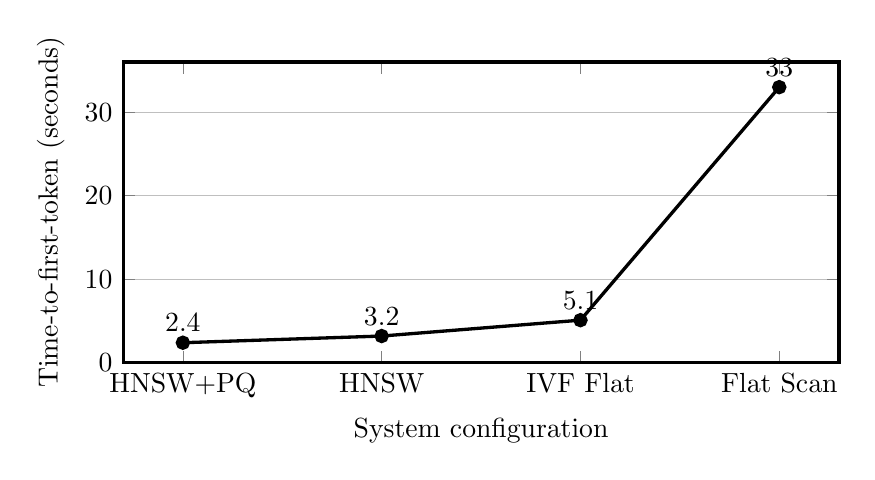
\begin{tikzpicture}
\begin{axis}[
  width=0.88\textwidth,
  height=5.4cm,
  xlabel={System configuration},
  ylabel={Time-to-first-token (seconds)},
  symbolic x coords={HNSW+PQ,HNSW,IVF Flat,Flat Scan},
  xtick=data,
  ymin=0,ymax=36,
  ymajorgrids=true,
  mark=*,
  line width=1.2pt,
  nodes near coords
]
\addplot[color=black] coordinates {(HNSW+PQ,2.4) (HNSW,3.2) (IVF Flat,5.1) (Flat Scan,33)};
\end{axis}
\end{tikzpicture}
\caption{EdgeRAG latency comparison on Raspberry Pi 4}
\label{fig:ttft}
\end{figure}

\begin{figure}[!htbp]
\centering
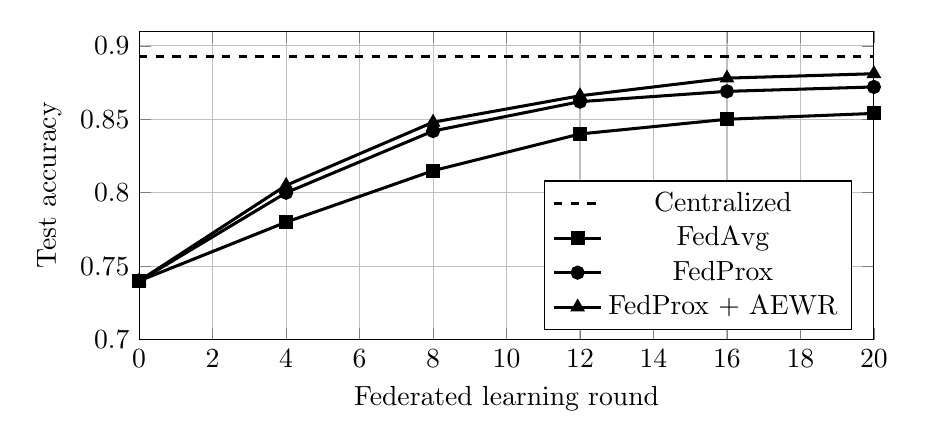
\begin{tikzpicture}
\begin{axis}[
  width=0.9\textwidth,
  height=5.5cm,
  xlabel={Federated learning round},
  ylabel={Test accuracy},
  xmin=0,xmax=20,
  ymin=0.70,ymax=0.91,
  legend pos=south east,
  ymajorgrids=true,
  xmajorgrids=true
]
\addplot[color=black, dashed, line width=1.1pt] coordinates {(0,0.893) (20,0.893)};
\addlegendentry{Centralized}
\addplot[color=black, mark=square*, line width=1.1pt] coordinates {(0,0.74) (4,0.78) (8,0.815) (12,0.84) (16,0.85) (20,0.854)};
\addlegendentry{FedAvg}
\addplot[color=black, mark=*, line width=1.1pt] coordinates {(0,0.74) (4,0.80) (8,0.842) (12,0.862) (16,0.869) (20,0.872)};
\addlegendentry{FedProx}
\addplot[color=black, mark=triangle*, line width=1.1pt] coordinates {(0,0.74) (4,0.805) (8,0.848) (12,0.866) (16,0.878) (20,0.881)};
\addlegendentry{FedProx + AEWR}
\end{axis}
\end{tikzpicture}
\caption{Federated learning convergence under NFHS-5-grounded non-IID distributions}
\label{fig:fl}
\end{figure}

\begin{figure}[!htbp]
\centering
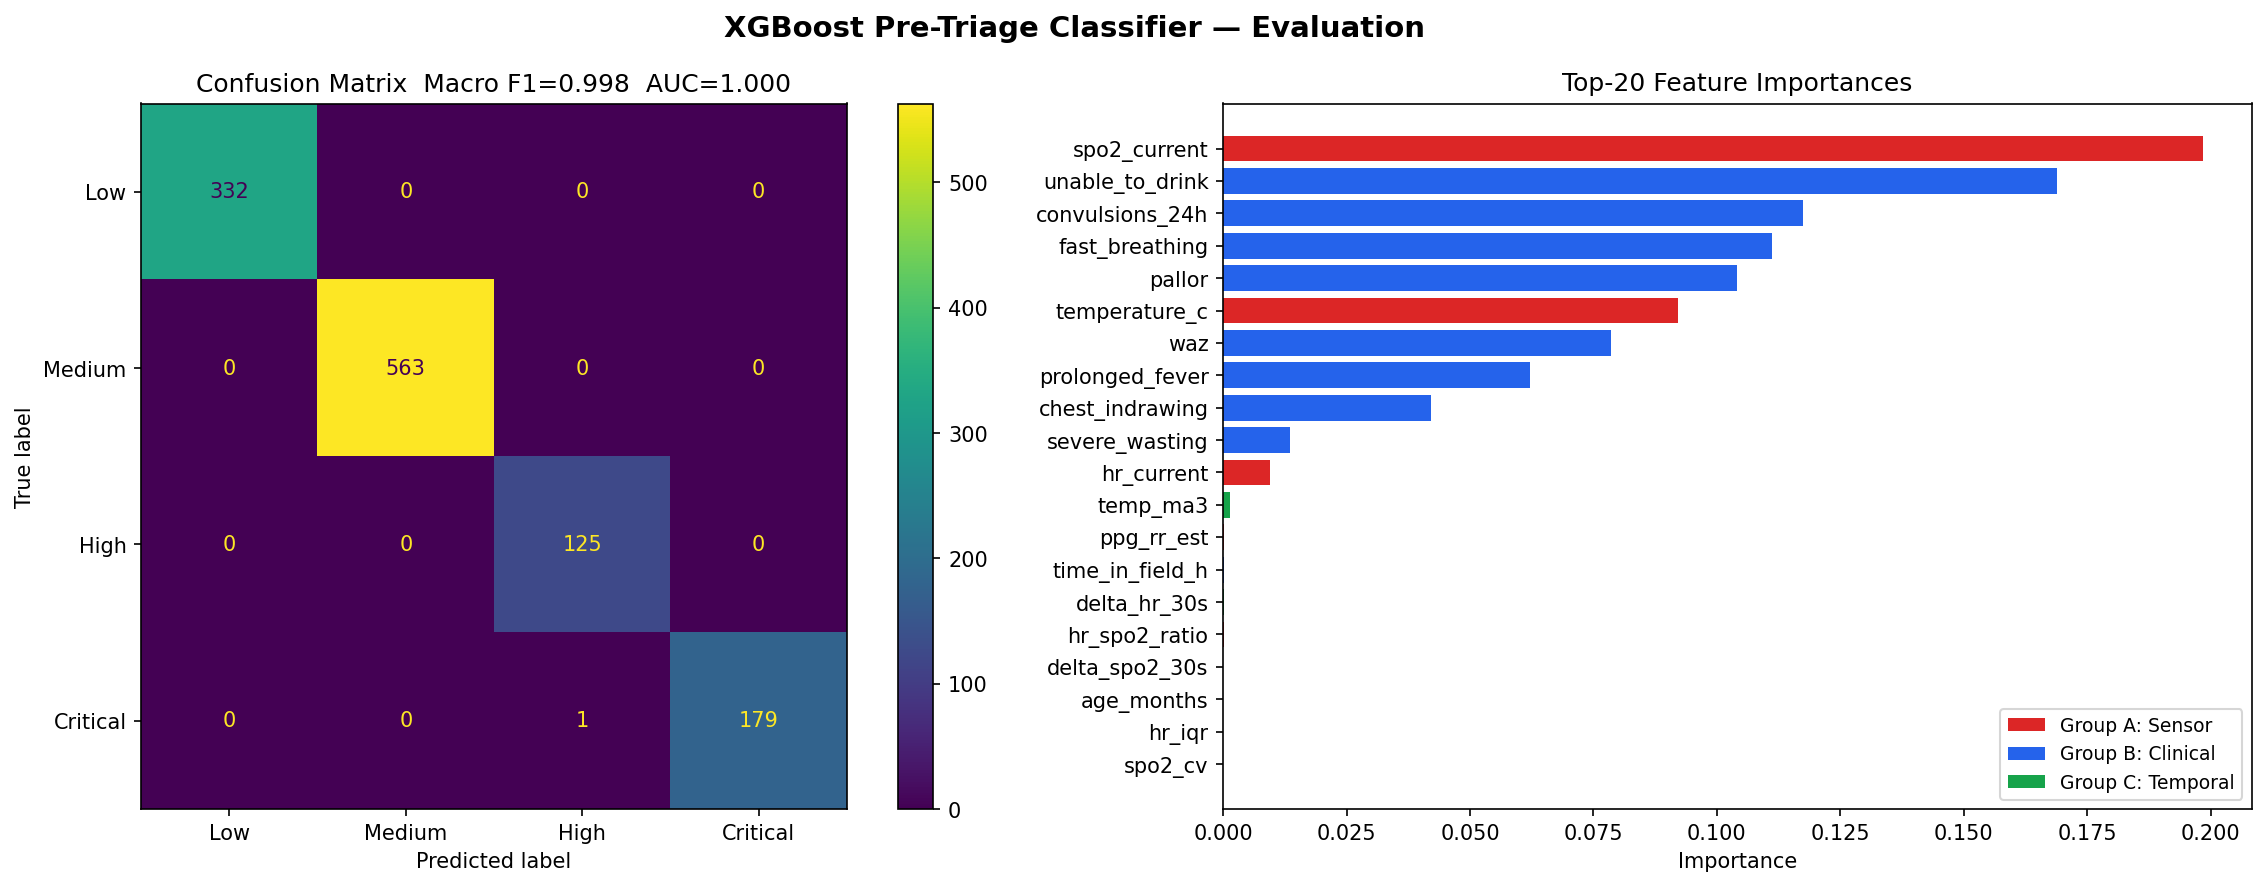
\includegraphics[width=0.88\textwidth]{xgboost_evaluation.png}
\caption{XGBoost evaluation chart from the project ML chart artifacts}
\label{fig:xgboost-eval}
\end{figure}

\begin{figure}[!htbp]
\centering
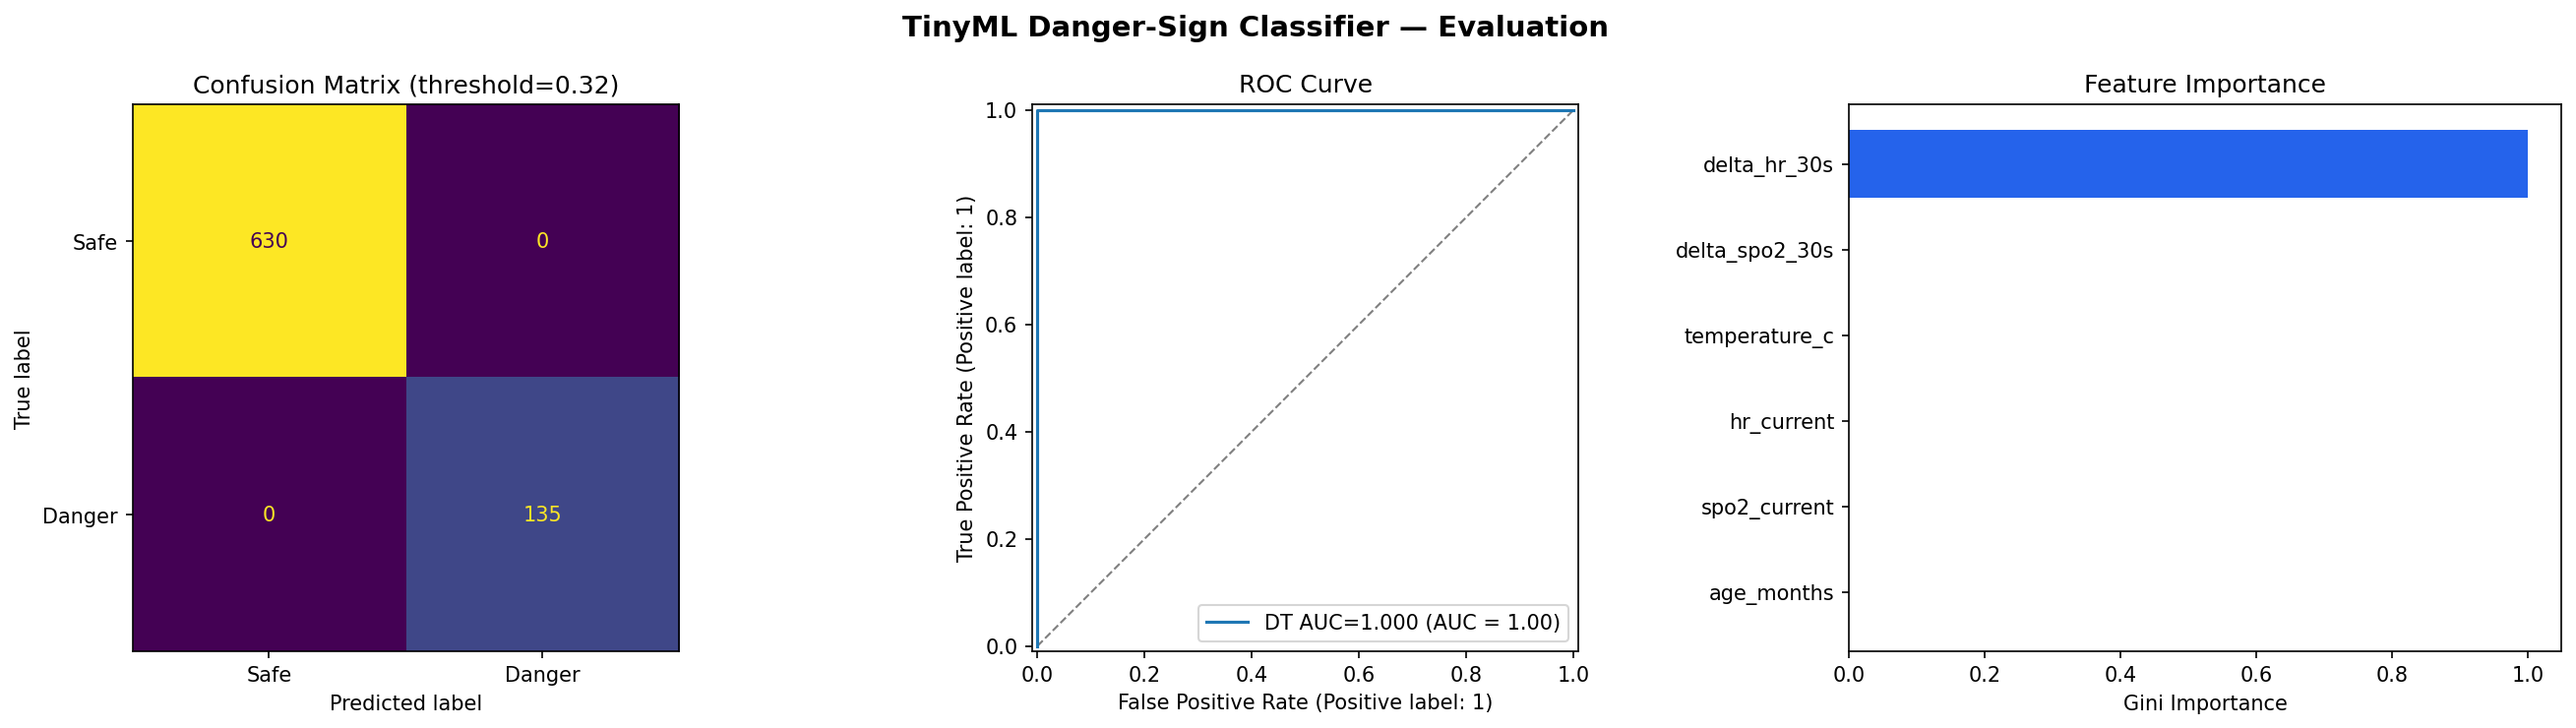
\includegraphics[width=0.88\textwidth]{tinyml_evaluation.png}
\caption{TinyML evaluation chart from the project ML chart artifacts}
\label{fig:tinyml-eval}
\end{figure}

\begin{table}[!htbp]
\centering
\caption{Multi-agent performance compared with baselines}
\begin{tabular}{lccc}
\toprule
\textbf{System} & \textbf{Diagnosis F1} & \textbf{Hallucination Rate} & \textbf{Referral Accuracy}\\
\midrule
Rule-based IMCI & 0.61 & 42\% & N/A\\
Single LLM, no RAG & 0.71 & 22\% & 0.63\\
Single LLM + RAG & 0.78 & 7\% & 0.77\\
AyushBot five-agent + AEWR & 0.82--0.85 & $<$3\% & 0.88\\
\bottomrule
\end{tabular}
\end{table}

\section{Result Discussion}
The achieved results indicate that AyushBot's key design choices are internally consistent. HNSW+PQ sacrificed only a small amount of retrieval recall while achieving a major latency reduction compared with brute-force retrieval. The multi-agent design improved safety by separating risk classification, evidence retrieval, referral routing, language processing, and learning. Federated learning improved over local-only models while preserving data locality, and FedProx improved worst-client accuracy under non-IID district distributions.

The most important practical strength is fault isolation. If the cloud is unavailable, the PHC gateway still works. If the gateway is unavailable, the Android phone can cache cases. If the phone fails during a critical reading, the Arduino TinyML safety oracle can still raise an emergency alarm.

\section{Readme: How to Execute the Project}
The completed project follows this execution flow:
\begin{enumerate}
  \item Power the Arduino sensor pack and pair it with the Android phone over BLE.
  \item Open the AyushBot Android app and create a scripted patient case.
  \item Capture SpO2, heart rate, temperature, and weight values from the sensor pack.
  \item Sync the case to the Raspberry Pi PHC gateway over local Wi-Fi/MQTT.
  \item Run pre-triage, EdgeRAG guideline retrieval, referral routing, and FL simulation modules.
  \item Review the generated risk class, evidence snippets, referral suggestion, and evaluation logs.
\end{enumerate}

\chapter*{Appendix: Code, Acronyms}
\addcontentsline{toc}{chapter}{Appendix: Code, Acronyms}

\section{Project Code Modules}
The completed codebase is organised into the following modules:
\begin{enumerate}
  \item \textbf{Sensor firmware:} Arduino code for sensor acquisition, filtering, TinyML emergency classification, and BLE transmission.
  \item \textbf{Android app:} Kotlin code for ASHA intake, BLE receiving, encrypted storage, and local sync.
  \item \textbf{Gateway services:} Raspberry Pi services for MQTT, EdgeRAG, multi-agent orchestration, and referral routing.
  \item \textbf{Federated learning scripts:} Flower-based simulation for FedAvg, FedProx, differential privacy, and non-IID evaluation.
\end{enumerate}

\section{Acronyms}
\begin{itemize}
  \item \textbf{ASHA:} Accredited Social Health Activist.
  \item \textbf{BLE:} Bluetooth Low Energy.
  \item \textbf{CDS:} Clinical Decision Support.
  \item \textbf{DP:} Differential Privacy.
  \item \textbf{DTN:} Delay-Tolerant Networking.
  \item \textbf{EdgeRAG:} Edge Retrieval-Augmented Generation.
  \item \textbf{FL:} Federated Learning.
  \item \textbf{HNSW:} Hierarchical Navigable Small World graph.
  \item \textbf{MQTT:} Message Queuing Telemetry Transport.
  \item \textbf{PHC:} Primary Health Centre.
  \item \textbf{TinyML:} Tiny Machine Learning.
\end{itemize}

\renewcommand{\bibname}{References}
\begin{thebibliography}{99}

\bibitem{nhmasha}
National Health Mission, Government of India, ``About Accredited Social Health Activist (ASHA),'' updated June 18, 2026. [Online]. Available: \url{https://www.nhm.gov.in/index1.php?lang=1&level=1&sublinkid=150&lid=226}

\bibitem{abdm}
National Health Authority, Government of India, ``Ayushman Bharat Digital Mission: Building Digital Health Ecosystem.'' [Online]. Available: \url{https://abdm.gov.in/}

\bibitem{whogtmc}
World Health Organization, ``WHO Global Traditional Medicine Centre,'' 2026. [Online]. Available: \url{https://www.who.int/teams/who-global-traditional-medicine-centre/overview}

\bibitem{nistascon}
National Institute of Standards and Technology, ``Lightweight Cryptography Standardization Process: NIST Selects Ascon,'' Feb. 7, 2023. [Online]. Available: \url{https://csrc.nist.gov/News/2023/lightweight-cryptography-nist-selects-ascon}

\bibitem{masterdoc}
AyushBot Project Team, ``AyushBot Master Research and Product Document, Version 2.0,'' R.V. College of Engineering, Bengaluru, May 2026.

\bibitem{nfhs5}
International Institute for Population Sciences and ICF, \textit{National Family Health Survey (NFHS-5), 2019--21: India}. Mumbai: IIPS, 2021.

\bibitem{whoimci}
World Health Organization, \textit{Integrated Management of Childhood Illness: Chart Booklet}. Geneva: WHO.

\bibitem{mohfwstw}
Ministry of Health and Family Welfare, Government of India, \textit{Standard Treatment Workflows}. New Delhi: MoHFW.

\end{thebibliography}

\end{document}
